\documentclass[a4paper,12pt]{article}
\usepackage{array}
\usepackage{amsmath}

\usepackage{graphicx} % Required for inserting images
\usepackage{amsmath,amssymb,amsfonts}
\usepackage{subcaption}
% Use Times New Roman font
\usepackage{times}
\usepackage[a4paper, top=1in, bottom=0.8in, left=1.1in, right=0.8in]{geometry}
\usepackage{float}
\usepackage{listings}
\usepackage{xcolor} % For customizing code colors
\setlength{\parindent}{0pt}
\usepackage{titlesec} % Add this to your preamble
\titleformat{\section}
{\normalfont\large\bfseries}{\thesection}{1em}{}
% Set spacing for sections
\titlespacing*{\section}
{0pt}  % Left spacing
{1ex} % Space before (adjust this value)
{1ex}  % Space after (adjust this value)
\begin{document}
	\section{Experiment No. 8}
	
	
	\section{Experiment Title }
	Design and analyze 4 Input logic gate ensuring proper DRC on MICROWIND 3.0
	\section{Objective}
	The main objectives of this report are:
	\begin{itemize}
		\item To design and analyze 4 Input logic gate using MICROWIND 3.0.
		\item To ensure proper compliance with Design Rule Check (DRC) requirements during the design process.
		
	\end{itemize}
	\section{Theory}
	\subsection{nMOS Inverter with Enhancement Mode (Pull-Up) Load}
	
	
	An nMOS inverter with an enhancement mode (pull-up) load consists of two nMOS transistors: the driving transistor (\(T_1\)) and the load transistor (\(T_2\)). The load transistor \(T_2\) is connected between the power supply \(V_{DD}\) and the output node, while \(T_1\) is connected between the output and ground. The gate of \(T_2\) is connected to \(V_{DD}\) to keep it ON when both inputs are low.\\
	\begin{figure}[H]
		\centering
		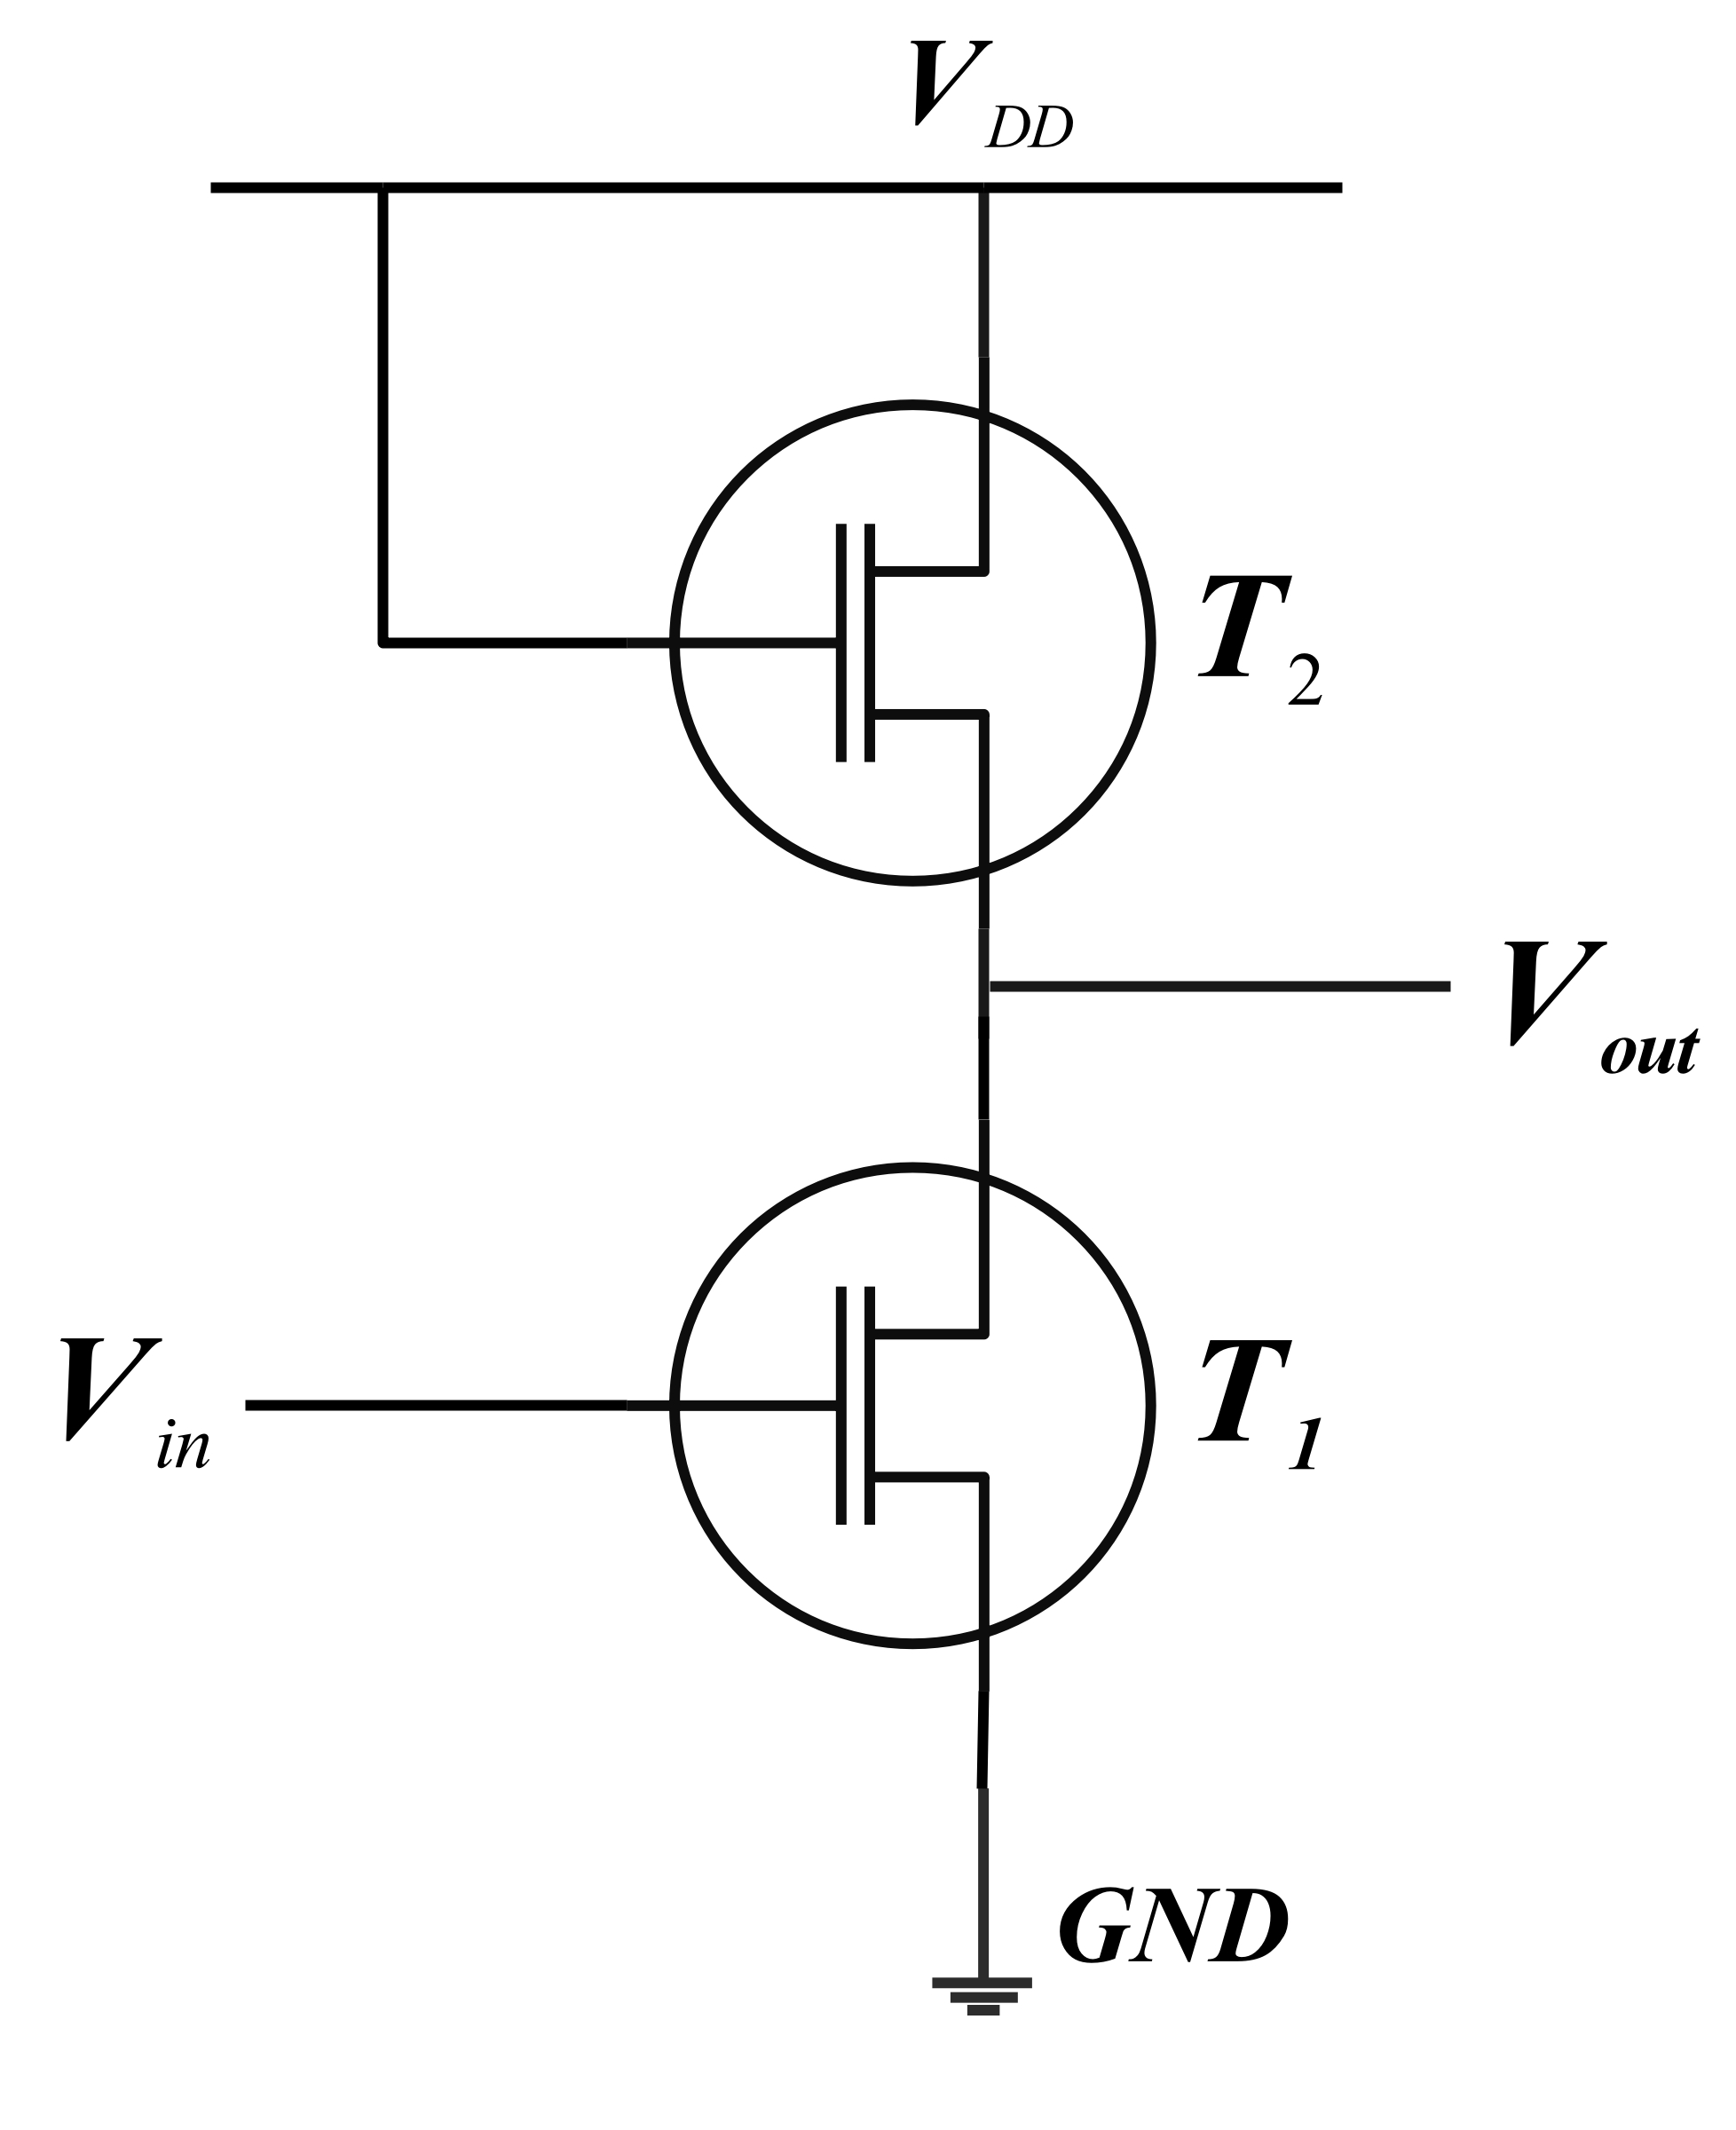
\includegraphics[width=0.45\linewidth]{../EXP04_EEE2214/Images/mos/1}
		\caption{nMOS Inverter with Enhancement Mode (Pull-Up) Load}
		\label{fig:1}
	\end{figure}
	
	- When the input \(V_{in}\) is low (logic '0'), \(T_1\) is OFF, and \(T_2\) pulls the output \(V_{out}\) high to \(V_{DD}\).\\
	- When \(V_{in}\) is high (logic '1'), \(T_1\) turns ON, pulling \(V_{out}\) low to 0V.
	\newpage
	\subsection{Proposed Boolean Expression:}
		\[
	Y = \overline{(A + A \cdot B + A \cdot B \cdot C \cdot D)}
	\]
	\subsection{Circuit Diagram}
	
	\begin{figure}[H]
		\centering
		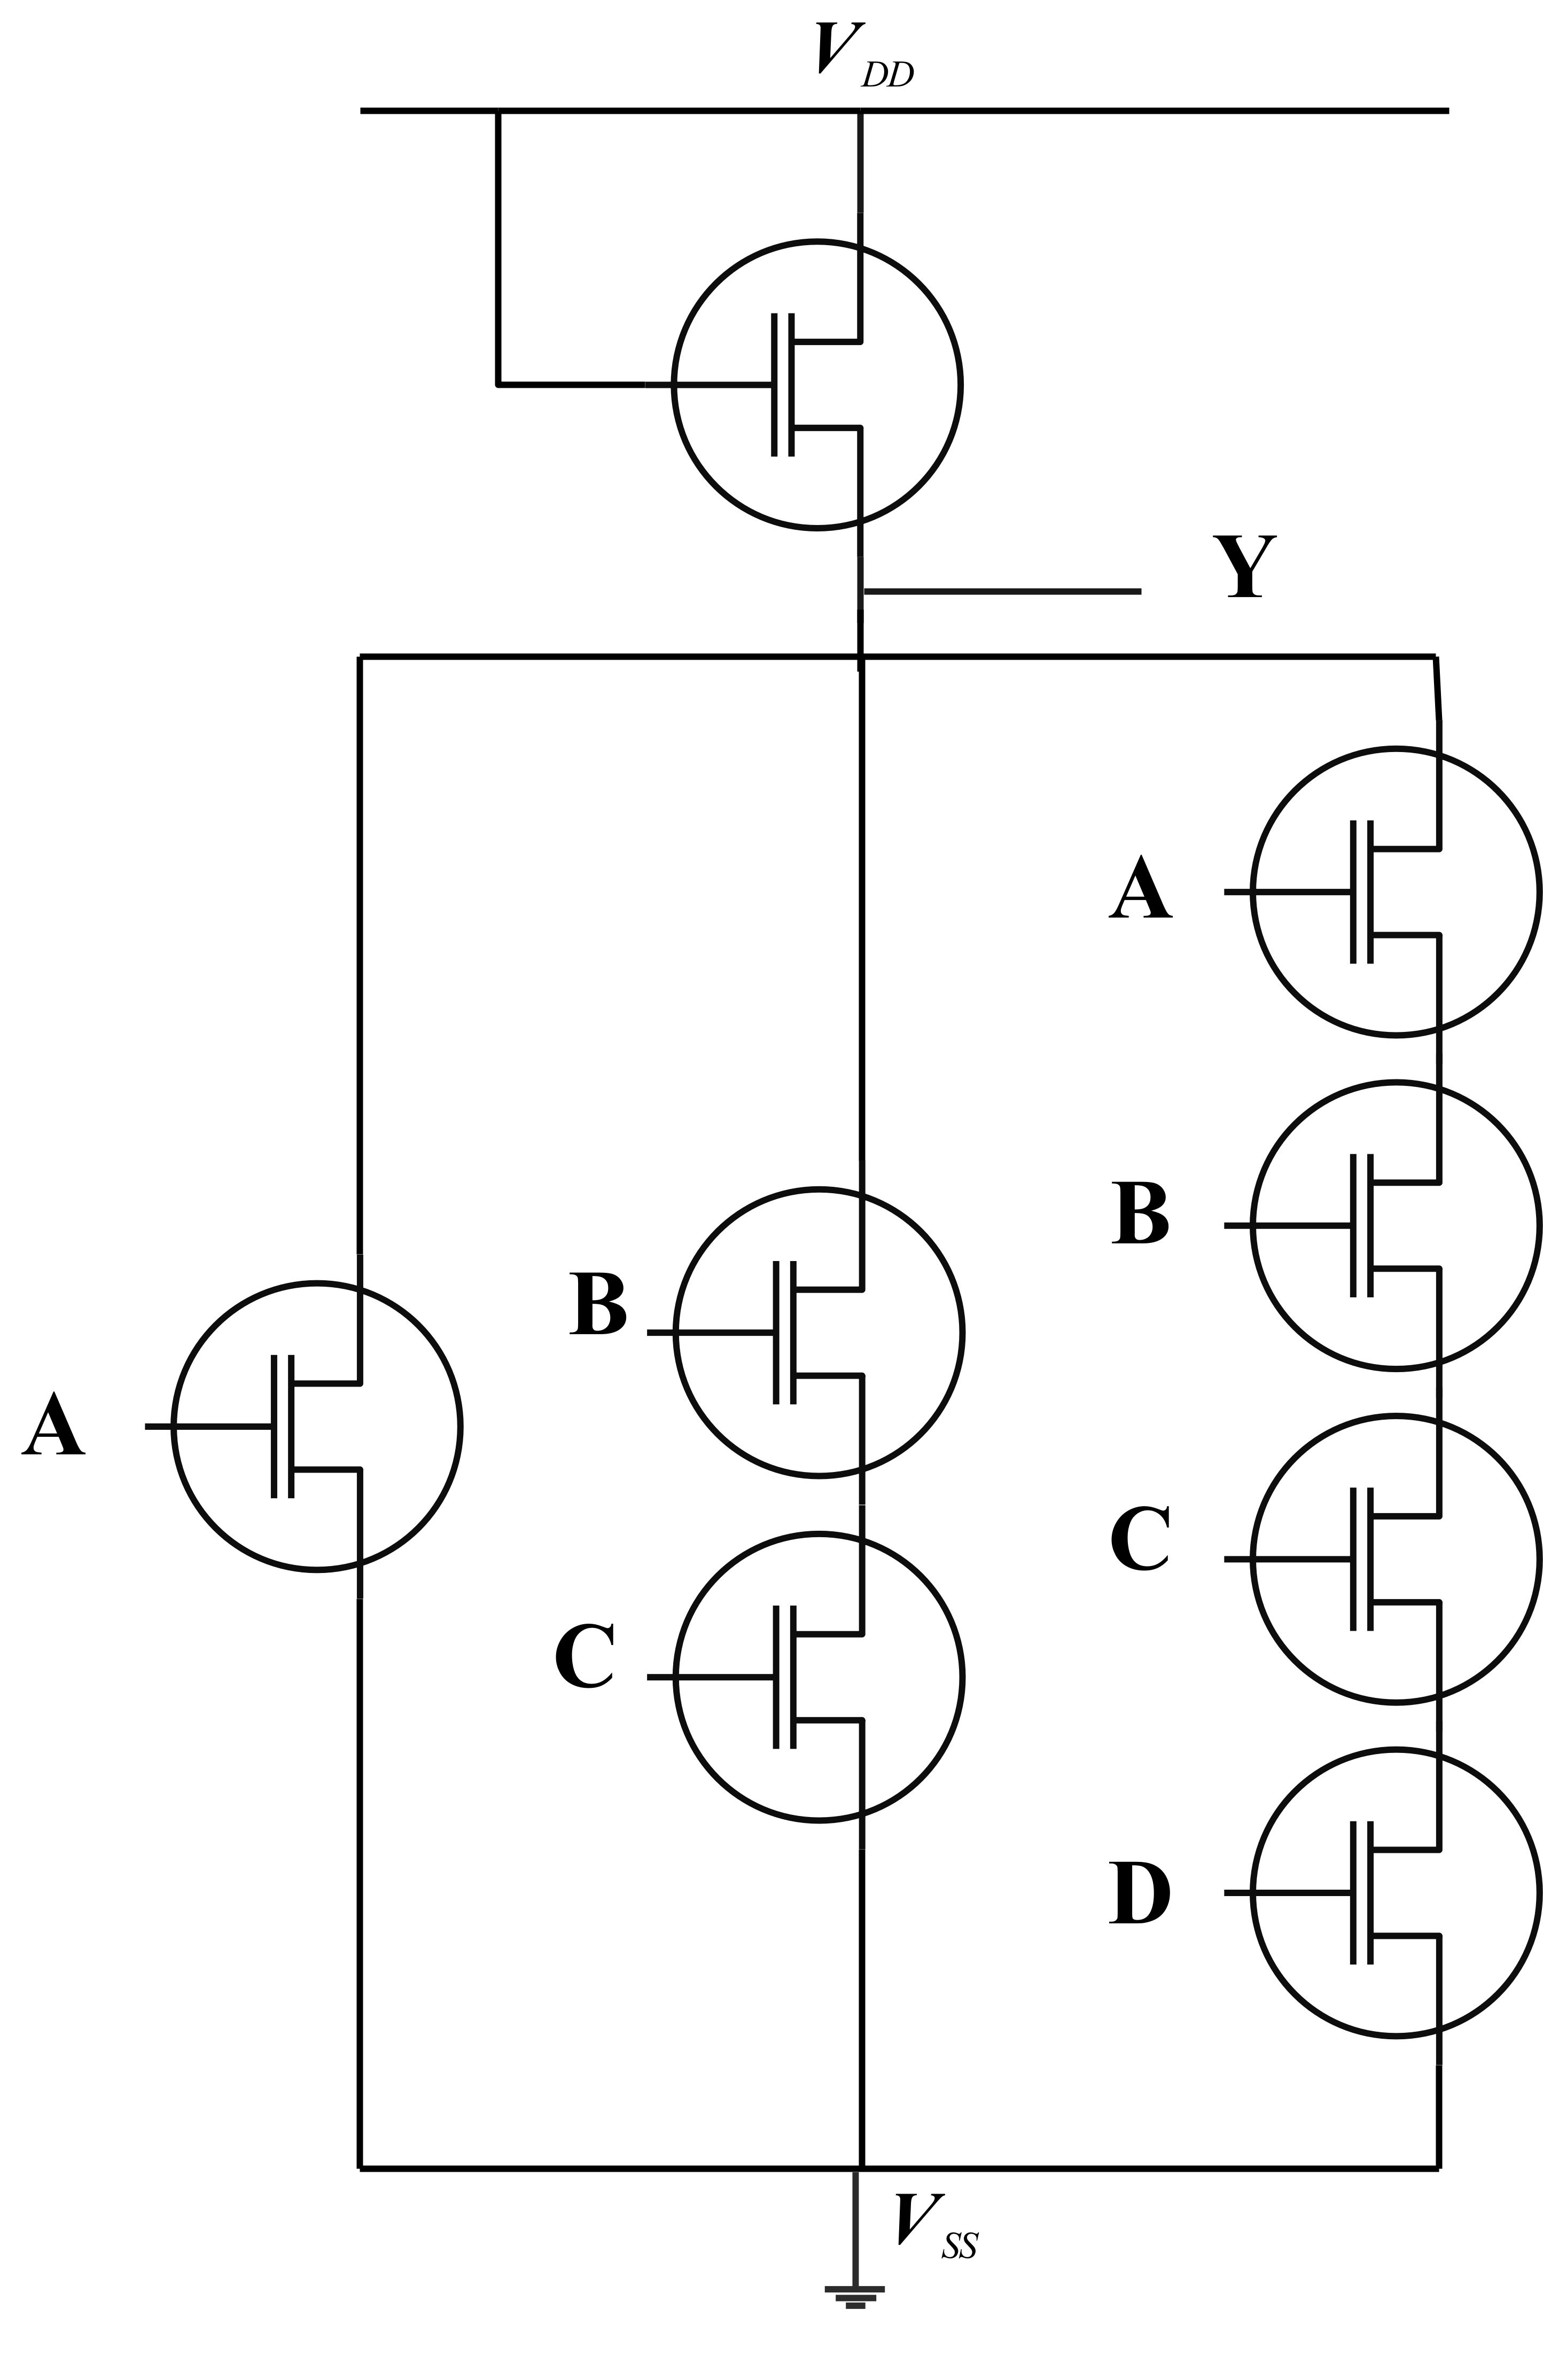
\includegraphics[width=0.4\linewidth]{Images/open}
		\caption{Y = $\overline{A + A . B + A . B . C . D}$}
		\label{fig:open}
	\end{figure}
	\subsection{Truth Table}
	

	\[
	\scalebox{1}{
	\begin{array}{|c|c|c|c|c|c|}
		\hline
		A & B & C & D & \text{Intermediate} & Y \\
		&   &   &   & A + A \cdot B + A \cdot B \cdot C \cdot D & \overline{(A + A \cdot B + A \cdot B \cdot C \cdot D)} \\
		\hline
		0 & 0 & 0 & 0 & 0 & 1 \\\hline
		0 & 0 & 0 & 1 & 0 & 1 \\\hline
		0 & 0 & 1 & 0 & 0 & 1 \\\hline
		0 & 0 & 1 & 1 & 0 & 1 \\\hline
		0 & 1 & 0 & 0 & 0 & 1 \\\hline
		0 & 1 & 0 & 1 & 0 & 1 \\\hline
		0 & 1 & 1 & 0 & 0 & 1 \\\hline
		0 & 1 & 1 & 1 & 0 & 1 \\\hline
		1 & 0 & 0 & 0 & 1 & 0 \\\hline
		1 & 0 & 0 & 1 & 1 & 0 \\\hline
		1 & 0 & 1 & 0 & 1 & 0 \\\hline
		1 & 0 & 1 & 1 & 1 & 0 \\\hline
		1 & 1 & 0 & 0 & 1 & 0 \\\hline
		1 & 1 & 0 & 1 & 1 & 0 \\\hline
		1 & 1 & 1 & 0 & 1 & 0 \\\hline
		1 & 1 & 1 & 1 & 1 & 0 \\\hline
		
	\end{array}}
	\]
	\newpage
	\section{Schematic Layout }
		\begin{figure}[H]
		\centering
		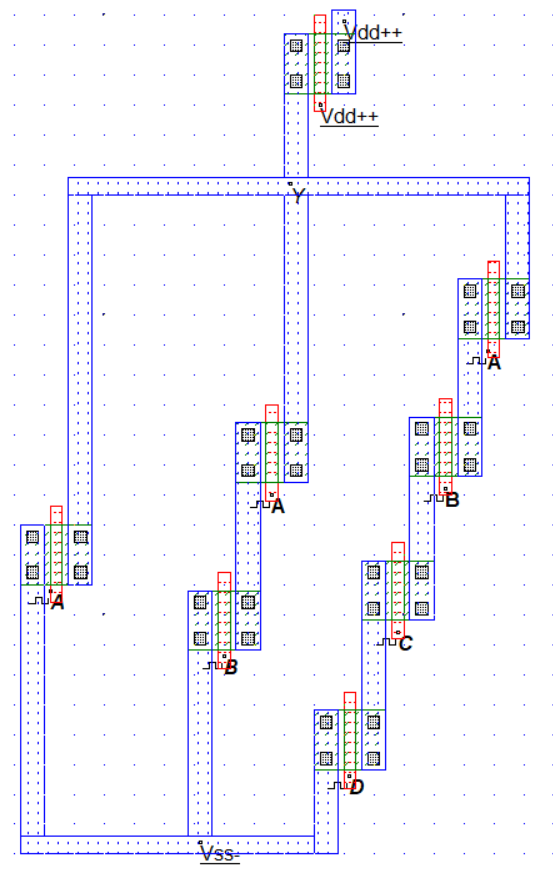
\includegraphics[width=0.9\linewidth]{Images/1}
		\caption{Y = $\overline{A + A . B + A . B . C . D}$ using nMOS Inverter with Enhancement Load}

		\label{fig:open}
	\end{figure}
	\section{Specification}
	\begin{table}[H]
		\centering
		\caption{MOSFET Dimensions for nMOS and pMOS Transistors}
		\label{tab:MOSFET_dimensions}
		\begin{tabular}{|c|c|c|c|c|}
			\hline
			\textbf{MOS} & \textbf{\begin{tabular}[c]{@{}c@{}}Width\\ ($\mu m$)\end{tabular}} & \textbf{\begin{tabular}[c]{@{}c@{}}Length\\ ($\mu m$)\end{tabular}} & \textbf{\begin{tabular}[c]{@{}c@{}}Width\\ ($\lambda$)\end{tabular}} & \textbf{\begin{tabular}[c]{@{}c@{}}Length\\ ($\lambda$)\end{tabular}} \\ \hline
			nMOS & 0.600 & 0.120 & 10 & 2 \\ \hline
		
		\end{tabular}
		
	\end{table}
	
	\begin{table}[H]
		\centering
		\caption{Parameters of Input Clock Signals for A,B,C \& D}
		% Sub-table (a)
		\begin{subtable}[t]{0.48\textwidth} % Adjusted width for each sub-table
			\centering
			\begin{tabular}{|c|c|c|}
				\hline
				\textbf{Parameter}          & \textbf{Value} & \textbf{Unit} \\ \hline
				High Level $(V)$            & 5.00           & $V$           \\ \hline
				Low Level $(V)$             & 0.00           & $V$           \\ \hline
				Time Low $(tl)$             & 0.225          & $ns$          \\ \hline
				Rise Time $(tr)$            & 0.002          & $ns$          \\ \hline
				Time High $(th)$            & 0.225          & $ns$          \\ \hline
				Fall Time $(tf)$            & 0.002          & $ns$          \\ \hline
			\end{tabular}
			\caption{Input clock signal of A} % Sub-table (a) caption
		\end{subtable}
		\hfil
		% Sub-table (b)
		\begin{subtable}[t]{0.48\textwidth} % Adjusted width for each sub-table
			\centering
			\begin{tabular}{|c|c|c|}
				\hline
				\textbf{Parameter}          & \textbf{Value} & \textbf{Unit} \\ \hline
				High Level $(V)$            & 5.00           & $V$           \\ \hline
				Low Level $(V)$             & 0.00           & $V$           \\ \hline
				Time Low $(tl)$             & 0.452         & $ns$          \\ \hline
				Rise Time $(tr)$            & 0.002          & $ns$          \\ \hline
				Time High $(th)$            & 0.452          & $ns$          \\ \hline
				Fall Time $(tf)$            & 0.002          & $ns$          \\ \hline
			\end{tabular}
			\caption{Input clock signal of B} % Sub-table (b) caption
		\end{subtable}
		
			\begin{subtable}[t]{0.48\textwidth} % Adjusted width for each sub-table
			\centering
			\begin{tabular}{|c|c|c|}
				\hline
				\textbf{Parameter}          & \textbf{Value} & \textbf{Unit} \\ \hline
				High Level $(V)$            & 5.00           & $V$           \\ \hline
				Low Level $(V)$             & 0.00           & $V$           \\ \hline
				Time Low $(tl)$             & 0.906          & $ns$          \\ \hline
				Rise Time $(tr)$            & 0.002          & $ns$          \\ \hline
				Time High $(th)$            & 0.906          & $ns$          \\ \hline
				Fall Time $(tf)$            & 0.002          & $ns$          \\ \hline
			\end{tabular}
			
			\caption{Input clock signal of C} % Sub-table (a) caption
		\end{subtable}
		\hfil
			\begin{subtable}[t]{0.48\textwidth} % Adjusted width for each sub-table
			\centering
			\begin{tabular}{|c|c|c|}
				\hline
				\textbf{Parameter}          & \textbf{Value} & \textbf{Unit} \\ \hline
				High Level $(V)$            & 5.00           & $V$           \\ \hline
				Low Level $(V)$             & 0.00           & $V$           \\ \hline
				Time Low $(tl)$             & 1.814          & $ns$          \\ \hline
				Rise Time $(tr)$            & 0.002          & $ns$          \\ \hline
				Time High $(th)$            & 1.814         & $ns$          \\ \hline
				Fall Time $(tf)$            & 0.002          & $ns$          \\ \hline
			\end{tabular}
			
			\caption{Input clock signal of D} % Sub-table (a) caption
		\end{subtable}
	\end{table}
	

	\begin{table}[H]
		\centering
		\caption{Parameters for Vdd+ and Vss- }
		\begin{tabular}{|c|c|c|}
			\hline
			\textbf{Parameter} & \textbf{Value} & \textbf{Unit} \\ \hline
			Vdd+               & 5.00           & $V $            \\ \hline
			Vss-               & 0.00           & $V$             \\ \hline
		\end{tabular}
		
	\end{table}
	
	\section{Output Waveshape }
		\begin{figure}[H]
		\centering
	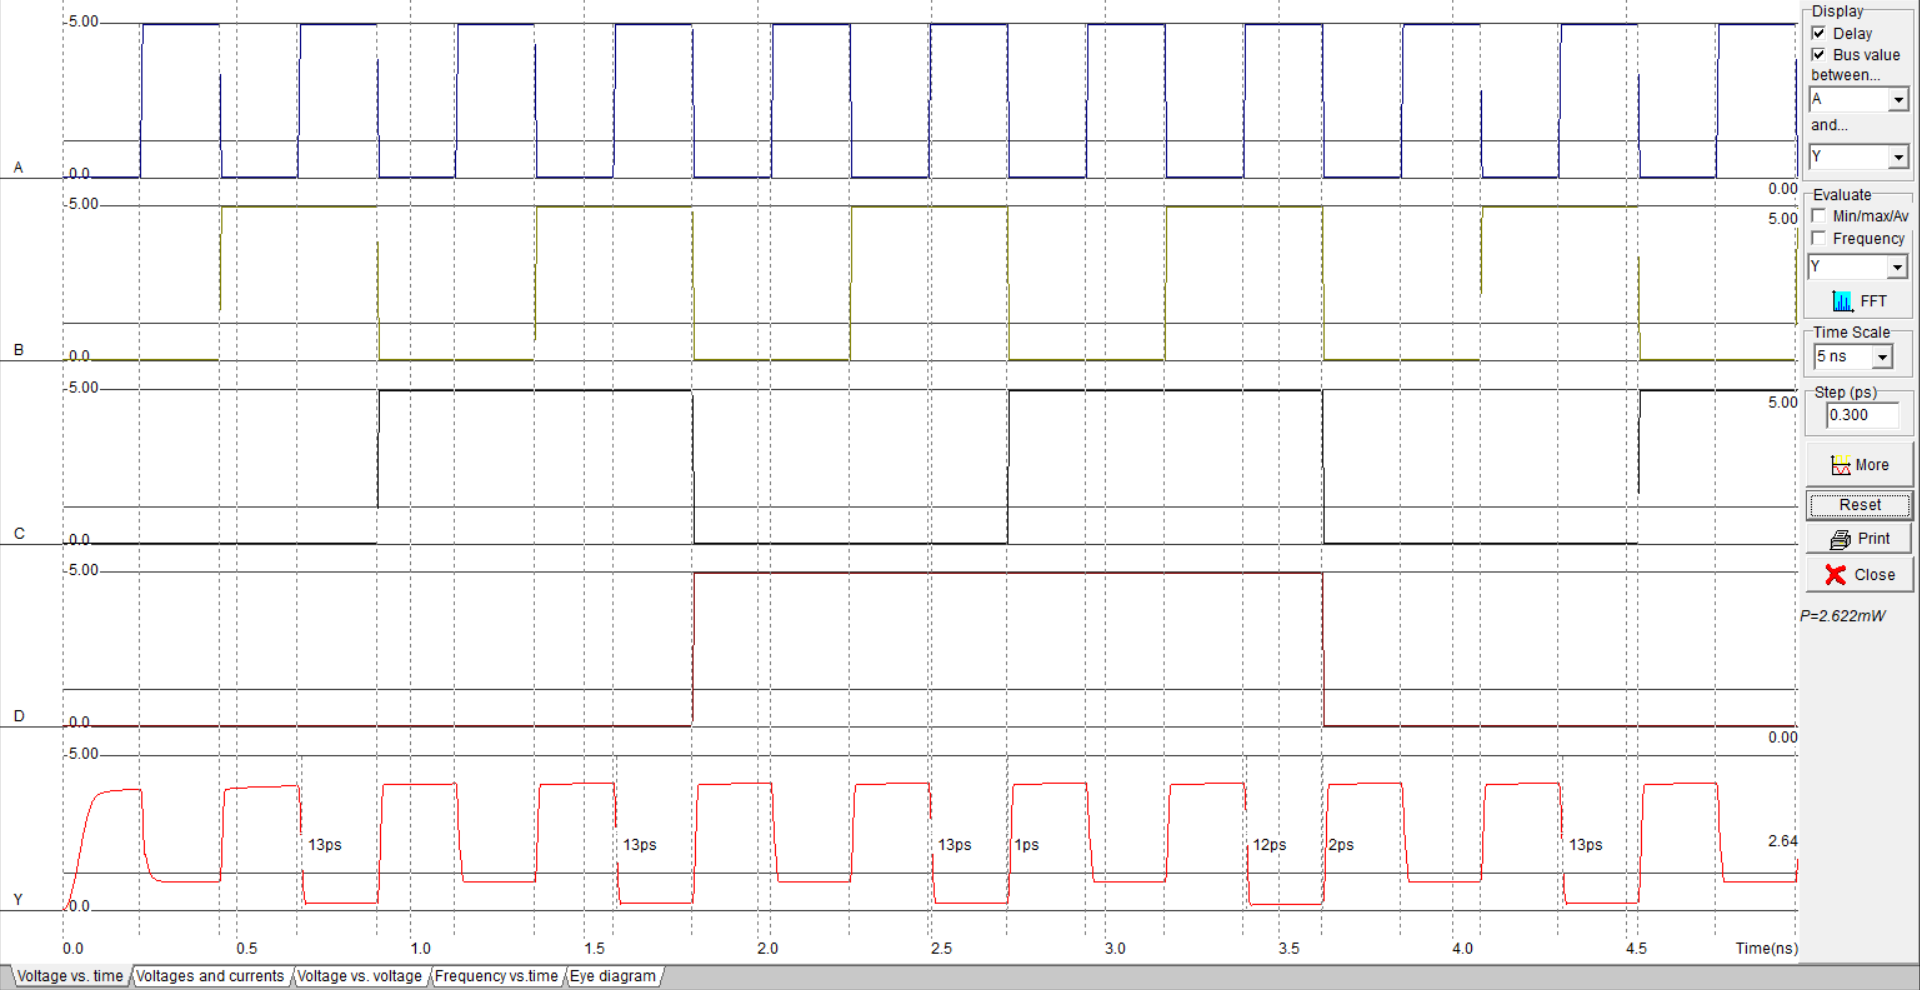
\includegraphics[width=1\linewidth, height=.45\textheight]{Images/2}
		\caption{Output Waveshape of 4 Input logic gate [Y = $\overline{A + A . B + A . B . C . D}$]}
		\label{fig:open}
	\end{figure}
	\section{Discussion }
	In the lab, we were tasked with designing and analyzing a 4-input logic gate while ensuring proper Design Rule Checking (DRC). 
	
	The proposed Boolean expression was:  
	\[
	Y = \overline{(A + A \cdot B + A \cdot B \cdot C \cdot D)} 
	\]
	For this Boolean expression, the circuit diagram, truth table, and waveform were designed before simulations. An nMOS inverter with an enhancement load was used for easier design implementation. \\	From the truth table, it was clearly observed that the output (\(Y\)) is the inverse of the input \(A\)'s clock signals. Specifically, when the input signal \(A\) was high, the entire circuit's output was low; conversely, when \(A\) was low, the output was high, even though there were three additional input signals with different frequencies.	The input signals were applied with different frequency to analyze the Boolean expression circuit according to the truth table. It was confirmed that the output accurately followed the predicted truth table.
	

\end{document}